% James Bradley's observation of light aberration (1725)
% Fig (a) shows an observation of a star on a non-moving Earth
% whereas Fig (b) shows an observation of a star on a moving Earth

\documentclass[tikz, border = 1 cm]{standalone}
\usepackage{tikz}

\usepackage{tkz-euclide}

\begin{document}
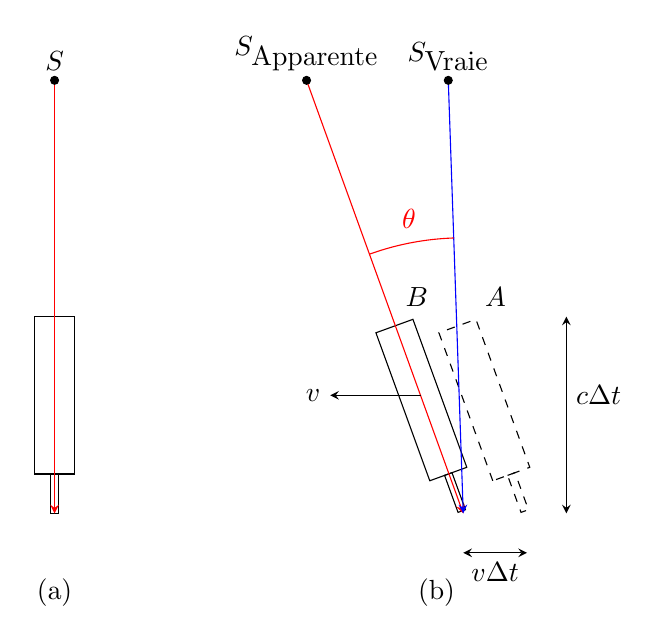
\begin{tikzpicture}
  % To draw the telescopes
      \newcommand{\telescope}[1][2]
                 {
                   \draw[#1] (-0.25,0) -- (-0.25,2) -- (0.25,2) -- (0.25,0) -- cycle;
                   \draw[#1] (-0.05,0) -- (0.05,0) -- (0.05,-0.5) -- (-0.05,-0.5) -- cycle;
                 }
                 
      %figure a
      \tkzDefPoint(0,5){E}

      \telescope[shift={(0,0)}, rotate=0];

      \draw[red,->,>=stealth] (E) -- (0,-0.5);

      \filldraw (E) circle (0.05);

      %The labels
      \node[above] at (E) {$S$};
      \node at (0,-1.5) {(a)};
      
      %figure b
      \tkzDefPoint(5,5){Strue} % The star at its true position
      
      \tkzDefPoint(3.2,5){Sapp} % The star at its apparent position
      \telescope[shift={(5,0)}, rotate=20];
      \telescope[shift={(5.8,0)}, rotate=20,dashed];
      \draw[red,->,>=stealth] (Sapp) -- (5.19,-0.5);
      \draw[blue,->,>=stealth] (Strue) -- (5.19,-0.5);

      \filldraw (Strue) circle (0.05);
      \filldraw (Sapp) circle (0.05);

      
      \draw[<->,>=stealth] (6.5,2) -- (6.5,-0.5);
      \draw[<->,>=stealth] (5.19,-1) -- (6,-1);
      \draw[<-,>=stealth] (3.5,1) -- (4.65,1);

      % The labels
      \node[above] at (4.6,2) {$B$};
      \node[above] at (5.6,2) {$A$};
      \node[above] at (Strue) {$S_{\textrm{Vraie}}$};
      \node[above] at (Sapp) {$S_{\textrm{Apparente}}$};
      \node[left] at (3.5,1) {$v$};
      \node[right] at (6.5,1) {$c\Delta t$};
      \node[below] at (5.595,-1) {$v\Delta t$};

      % The angle theta
      \begin{scope}
        \clip (Sapp)  -- (Strue) -- (5.19,-0.5) -- cycle;
        \draw [red] (5.19,-0.5) circle (3.5);
\node[above,red] at (4.5,3) {$\theta$};
      \end{scope}
      
      \node at (4.85,-1.5) {(b)};
    \end{tikzpicture}
\end{document}
